\def\year{2017}\relax
%%%% ijcai16.tex

% These are the instructions for authors for IJCAI-16.
% They are the same as the ones for IJCAI-11 with superficical wording
%   changes only.

\documentclass[letterpaper]{article}
% The file ijcai16.sty is the style file for IJCAI-16 (same as ijcai07.sty).
\usepackage{aaai17}
\usepackage{times}
\usepackage{helvet}
\usepackage{courier}
\usepackage{multirow}
\frenchspacing
\setlength{\pdfpagewidth}{8.5in}
\setlength{\pdfpageheight}{11in}
\pdfinfo{
%/Title (Efficient Online Optimized Model Adaptation by Incremental Simplex Tableau)
%/Author (Zhixian Lei, Yongcai Wang, Xuehan Ye)
%/Keywords (Online Learning, Model Adaption, Simplex)
}
\usepackage{amsmath, amssymb, amsthm}
\usepackage{graphicx}
\usepackage{subfigure}
\usepackage{algorithm}
\usepackage{algorithmic}
\usepackage[draft]{hyperref}
\usepackage{url}

\renewcommand\floatpagefraction{.9}
\renewcommand\topfraction{.9}
\renewcommand\bottomfraction{.9}
\renewcommand\textfraction{.1}
\setcounter{totalnumber}{50}
\setcounter{topnumber}{50}
\setcounter{bottomnumber}{50}

\setlength{\floatsep} {1pt plus 1pt minus 1pt}
\setlength{\textfloatsep} {1pt plus 1pt minus 1pt}

\renewcommand{\baselinestretch}{1.0}


% Use the postscript times font!
\usepackage{color}
\newtheorem{definition}{Definition}
\newtheorem{theorem}{Theorem}
\newtheorem{lemma}{Lemma}
\newtheorem{assumption}{Assumption}
\newtheorem{proposition}{Proposition}
\newtheorem{example}{Example}
\newtheorem{problem}{Problem}

% the following package is optional:
%\usepackage{latexsym}

% Following comment is from ijcai97-submit.tex:
% The preparation of these files was supported by Schlumberger Palo Alto
% Research, AT\&T Bell Laboratories, and Morgan Kaufmann Publishers.
% Shirley Jowell, of Morgan Kaufmann Publishers, and Peter F.
% Patel-Schneider, of AT\&T Bell Laboratories collaborated on their
% preparation.

% These instructions can be modified and used in other conferences as long
% as credit to the authors and supporting agencies is retained, this notice
% is not changed, and further modification or reuse is not restricted.
% Neither Shirley Jowell nor Peter F. Patel-Schneider can be listed as
% contacts for providing assistance without their prior permission.

% To use for other conferences, change references to files and the
% conference appropriate and use other authors, contacts, publishers, and
% organizations.
% Also change the deadline and address for returning papers and the length and
% page charge instructions.
% Put where the files are available in the appropriate places.

\title{Efficient Online  Model Adaptation by Incremental Simplex Tableau}
\author{Zhixian Lei$^1$, Xuehan Ye$^2$, Yongcai Wang$^2$\footnotemark,   Deying Li$^2$, Jia Xu $^3$\\
$^1$ Department of Computer Sciences, Harward University, USA; \\$^2$ Department of Computer Sciences, Renmin University of China, Beijing; \\$^3$ Department of Computer Sciences, City University of New York, USA
}



\begin{document}

\maketitle
\footnotetext{corresponding author: Yongcai Wang, ycw@ruc.edu.cn}

\begin{abstract}
Online multi-kernel learning is promising in the era of mobile computing, in which a combined classifier with multiple kernels are offline trained, and online adapts to personalized features for serving the end user precisely and smartly. The online adaptation is mainly carried out at the end-devices, which requires the adaptation algorithms to be light, efficient and accurate. Previous results focused mainly on efficiency.
This paper proposes an novel online model adaptation framework for not only efficiency but also optimal online adaptation.

At first, an online optimal \emph{incremental simplex tableau (IST)} algorithm is proposed, which approaches the model adaption by linear programming and produces the optimized model update in each step when a personalized training data is collected.
But keeping online optimal in each step is expensive and may cause over-fitting especially when the online data is noisy. A  \emph{Fast-IST} approach is therefore proposed, which  measures the deviation between the training data and the current model. It schedules updating only when enough deviation is detected. The efficiency of each update is further enhanced by running IST only limited iterations,  which bounds the computation complexity. Theoretical analysis and extensive evaluations show that Fast-IST saves computation cost greatly, while achieving speedy and accurate model adaptation.  It provides better model adaptation speed and accuracy while using even lower computing cost than the state-of-the-art.
\end{abstract}

\section{Introduction}
Online adaptive learning is widely required in the era of mobile and wearable computing\cite{SongSurvey}, in which a classifier, generally trained offline, needs to adapt to the personalized features after being delivered to end users. The goal is to serve the end users precisely and smartly \cite{Gu20051}.

% The model needs to  using limited training data cannot cover the personalized and temporary features of all the potential users at any time. Given a model regularized for vast majority of samples, we need to update the model online after a particular user using the application, for providing precise services to the end users . %Here, we focus our updating scheme to changing the weights for different features of the data in real time. The weights represent the importance attached to different features by the model which reflects the anticipation of the data.

Challenges are posed from three aspects: 1) the online model adaptation is mainly carried out at the end devices, requiring the adaptation algorithms to be efficient for energy efficiency etc. 2) The personalized online training data is generally noisy, challenging the adaptation speed and the risk of over-fitting.
 3) The training data comes from multiple sources or in different metric spaces, requiring adaptive feature selection and weighting \cite{hong2009context}.



%Therefore adaptive feature weighting and online model adaptation need to be jointly considered.
Model learning from multiple features of different metric spaces, was traditionally, mainly studied  in offline feature selection \cite{6788385} \cite{Huang2005325}. % by sensitivity analysis \cite{Shen:2008}, filtered sequential forward search \cite{Liu20061333}, kernel polarization \cite{6788385} and mutual information minimization \cite{Huang2005325}\cite{graph}\cite{Foithong2012574} methods.
Automatic and adaptive feature weighting was proposed by multi-kernel learning (MKL)\cite{Sonnenburg:2006} \cite{Gonen:2011}, which learns an optimal linear or non-linear combination of a set of predefined kernels to reduce the bias of manually weighting.

The flexibility of adaptively multiple feature weighting by combining multiple kernels enables recent studies for online multiple kernel learning (OMKL) \cite{martins2011online}\cite{Hoi2012}\cite{Wang2015124}. OMKL generally composes two online learning sub-problems: 1) \emph{perception} \cite{Freund:1999:LMC:337859.337869} , to train a basic classifier (BC) for each given kernel; and 2) \emph{combination}, which is to weight and combine the BCs to generate a combined, more accurate classifier. Since the training of the BCs and the optimization of the combining weights for BCs are generally coupled, which involves quadratic programming\cite{Lanckriet01112004} or semi-infinite linear programming \cite{Sonnenburg:2006}\cite{Rakotomamonjy:2007}, OMKL is generally computation extensive,  even in offline training. Therefore, seeking efficiency is the major focus of current OMKL algorithms.


A major approach for efficiency is to decouple the perception and the classifier combination steps by training the BCs offline. This reduces the online learning problem to only adapt the combination weights based on the online training data \cite{Incremental} \cite{Luo} \cite{jin2010}. The key idea is to increase the weights for the BCs whose outputs coincide with the online collected training data, and to decrease if inconsistent \cite{chaudhuri2009parameter}\cite{Incremental}. %deterministic updating and stochastic updating.

But a key challenge of focusing on efficiency is the lack of guarantee on the responding speed.  Like in \emph{hedge}\cite{chaudhuri2009parameter}\cite{Freund1997119}, the model coefficients are updated only one time when a training data is applied. The accurate adaptation thus requires corrections by many training instances, leading to slow adaptation.  This paper, instead,  seeks efficient, speedy, and optimal online adapation.  It at first proposes an incremental simplex tableau (IST) algorithm, which can produce the optimal linear weights in each step based on the online collected training data. It is in practice carried out by simple row and column operations in the simplex tableau \cite{Schrijver:1986:TLI:17634}. The intuition is that the tableau saves the previous optimal state, and the new optimal is generally not far from the old optimal, which can be achieved quickly.

But keeping optimal in each step is expensive and not necessary, especially when the training data is noisy. A Fast-IST framework is therefore developed for efficiency and noise tolerance. It uses a mini-batch, fixed-iteration online adaptation strategy \cite{bottou1998online}. The online training data are organized into batches. Only when the majority of samples in a batch are far from the current model, will the algorithm update the model by fixed-iteration IST, i.e., fixed steps of simplex operations. In this way, the frequency of updating is reduced; the possible wrong samples are filtered; and the cost in each updating is bounded.  Analysis and evaluations by both simulations and experimental data showed that Fast-IST provided better classification accuracy and speedy responding than the current OMKL approaches\cite{Freund1997119}\cite{chaudhuri2009parameter}, using even less computation costs. % Fast-IST also requires comparable computing cost comparing with the heuristic algorithms.



%\cite{MartinsSXAF11}\cite{review}\cite{Hoi2012}\cite{Wang2015124} \color{blue} problems of online MKL and our advantages than online MKL.


%Further, the offline training is based on limited dataset, which cannot fully cover the feature variations of all potential users. So the trained model is not precise for individual user, degrading the prediction accuracy especially for the users whose features deviate from the common features seen from the training set.

%Existing approaches investigated mutual information minimization \cite{Huang2005325}\cite{graph}\cite{Foithong2012574} to find the representative features, but accurate evaluation of mutual information need to collect large amount of instances, which is not agile in online phase.
%Similarity based online feature selection \cite{1593673} requires the training data contains both positive and negative sets. Existing works also proposed online multiple kernel learning algorithms \cite{MartinsSXAF11}\cite{Incremental}\cite{review}\cite{jin2010}\cite{Hoi2012}\cite{Wang2015124} \color{blue} problems of online MKL and our advantages than online MKL.
%\color{black}

The rest of the paper is organized as following. Problem model and preliminaries are introduced in Section 2. IST is introduced in Section 3. Fast-IST is introduced in Section 4. Property analysis and performance evaluations are summarized in Section 5. The paper is concluded with remarks in Section 6.

\section{Problem model and Preliminaries}
%The problem model and the background of \emph{simplex} and \emph{dual simplex} algorithms are introduced in this section.

This paper considers a general application scenario of OMKL, where a classifier composed by linear combination of multiple basic classifiers (BC) have been offline trained. We want the model, i.e., the linear weights, can online adapt to personalized data when the classifier is used by a user. %Conceivably the distribution of personalized data might be different from global data and might change over time.
The goal is to make the adaptation quick and use less computation cost. %combine the basic classifiers in a smart way to fit personalized data and online updating this model given the personalized data as a stream.
Since the multi-class classification problem can be transformed to binary classification by constructing a binary tree, for simplicity of exposition, we focus on binary classification in this paper.

Considering personalized data is arriving in a stream $(\mathbf{x}_1, y_1), (\mathbf{x}_2, y_2), \ldots$,  where $\mathbf{x}_i$  is the $i$th feature data and $y_i$ is the corresponding class label: $y_i \in \{-1, 1\}$. The set of BCs is $\{G_j : G_j(\mathbf{x}) \in \{-1, 1\}, j \in [m]\}$ where $G_j(\mathbf{x_i})$ is a prediction of $y_i$. After receiving $n$th data, ideally we hope to find suitable combining weights $\{a_j : j \in [m]\}$ such that the combined classifier can produce better classification than the offline trained one. The combined classifier is:
\begin{equation}
G(x) = \textrm{sign}\left[\sum_{j=1}^m a_jG_j(\mathbf{x})\right]
\label{eqn:model}
\end{equation}
where $[n]$ and $[m]$ denote $\{1, 2, \ldots n\}$ and $\{1, 2 \ldots, m\}$ respectively. %For example, $G_j$ can be different classification algorithms and $G$ is a combined algorithm or different $G_j$ use different parts of $\mathbf{x}_i$ and $G$ can make full use of training data.
Since all $G_j$s are BCs offline trained, we assume $G_j$ can classify $x_i$ correctly with probability higher than $50\%$, which is more powerful than random prediction.



%In this paper, we focus on giving algorithm which is fast for online updating $G$. In other word, we want to find new $G$ from existing $G$ efficiently when adding new data or deleting past data. Note that for multi-class classification problem, we can transform it to binary classification by constructing a binary tree from those classes. More specifically, we take those classes as leaf nodes and construct a binary tree from bottom to top where each time we create a parent node from two child nodes in the sense that these two child nodes share similar features.
%
%Note that for multi-class classification problem, we can transform it to binary classification by constructing a binary tree, those classes as leaf nodes and construct a binary tree from bottom to top where each time we create a parent node from two child nodes in the sense that these two child nodes share similar features.

The model adaptation can be transformed into an optimization problem. We seek  $\forall j\in [m], a_j \geq 0$ and $\sum_{j=1}^m a_j = 1$, such that the following objective is minimized:
\begin{align}
\textrm{minimize: } & \sum_{i=1}^n \epsilon_i
\label{model}
\end{align}
\vspace{-0.5cm}
\begin{align*}
\small
\textrm{subject to: }
& y_i\sum_{j=1}^m a_jG_j(\mathbf{x}_i) \geq - \epsilon_i & \forall i \in [n]\\
& \epsilon_i \geq 0 & \forall i \in [n]
\label{eqn:lp}
\end{align*}
where $\{\epsilon_i : i \in [n]\}$ is the possible error of the combined new classifier $G$. %Since $a_j \geq 0~ \forall j \in [m]$ and $\sum_{j=1}^m a_j = 1$, it has $0 \leq a_j \leq 1$ and $\lVert \mathbf{a} \rVert$ can not be much large.

Note that, the optimal $G$ from this linear programming should have less training error than any $G_j$, i.e.,  providing not worse prediction accuracy for $\mathbf{x}_i$, since we can always achieve $G = G_j$ by assigning $a_j = 1$ and $a_i = 0~\forall i \in [m], i \neq j$. %, when $m$ is large, in general we can find $G$ with very low error probability when predicting $\mathbf{x}_i$.
\begin{theorem}
If basic classifiers predicts independently and randomly, the prediction error of the optimal $G$ decreases exponentially with $m$.
\end{theorem}
\begin{proof}
Suppose $\forall j \in [m]$, $G_j$ randomly predicts with correct probability $p_j > 1/2$. Then the expectation $\mathbb{E}[y_iG_j(\mathbf{x}_i)] = p_j - (1 - p_j) = 2p_j - 1$ and
\begin{equation}
\mathbb{E}\left[y_i\sum_{j=1}^m a_jG_j(\mathbf{x}_i)\right] = \sum_{j=1}^m a_j(2p_j - 1)
\end{equation}
If we take $a_j = 1/m~\forall j \in [m]$ and let $\sum_{j=1}^m (2p_j - 1)a_j = 2p^* - 1$, by Hoeffding's inequality, the probability for incorrect prediction on $(\mathbf{x}_i, y_i)$ is
\begin{equation}
 \Pr\left[y_i\sum_{j=1}^m a_jG_j(\mathbf{x}_i)< 0\right] \leq e^{-\Omega(m(2p^* - 1)^2)}
\end{equation}
%Since $a_j = 1/m~\forall j \in [m]$ is a feasible assignment for $a_j$, the optimal $G$ should make wrong prediction with probability exponentially small in $m$.
Thus, the theorem holds.
\end{proof}
This theorem provides some worst case analyses for our mechanism when all basic classifiers are independent and random. The effectiveness of the algorithm in these settings in general demonstrates a better performance in real life application.
% \begin{theorem}
% The offline linear programming can return the optimal weights to form an optimized combined classifier $G$ for the training data.
% \end{theorem}
% \begin{proof}
% Because the linear programming model in (2) is a convex optimization problem, the optimal solution can be therefore achieved by linear programming.
% \end{proof}

The key problem for online learning is to adapt the model weights efficiently and correctly. This contains two folds: 1) an efficient online model adapation algorithm; 2) efficient  online data preprocessing to schedule the model update to avoid high computation cost and over-fitting. Solutions to these two problems are presented as following:



%For efficiency, a fast algorithm to approximate optimal solution in each update is needed for online setting. For correctness, we consider that not all data points represent true state and label since there exists potential noise. To achieve above goals, we formulate two corresponding problems:
%\begin{problem}[Data Filtering]
%Given the training data $\{(\mathbf{x}_i, y_i), i\in[n]\}$, can we reduce the workload of learning algorithm by filtering the evident correct data points (not necessary for model to change) and evident wrong data points (interfering data from noise)?
%\end{problem}
%\begin{problem}[Online adapting]
%Given the offline trained optimal classifier $\{a_j\}, \{G_j\}, j\in[m]$ and the training data $(\mathbf{x}_i, y_i), i\in[n]$ after filtering, can we quickly find nearly optimal solution for linear programming from previous solution in last updating?
%\end{problem}

%\subsection{Relation to Multi-kernel Learning}
%The \emph{multi-kernel learning} model is very similar to the investigated problem and can be reduced to the model. Given a set of training data $\{(\mathbf{x}_i, y_i) : y_i \in \{-1, 1\}, i \in [n]\}$ and a set of kernel functions $\{\mathbf{K}_j : j \in [m]\}$, the multi-kernel learning problem aims to find the optimal combination of kernel function $\mathbf{K} = \sum_{j=1}^m a_j\mathbf{K}_j$, where $\sum_{j=1}^m a_j = 1$, to minimizes the classification error.
%% and the classification error can be formulated as the objective of the following optimization problem:
%%\begin{align*}
%%\textrm{maximize: } & \sum_{i=1}^nb_i - \frac{1}{2}\sum_{i=1}^n\sum_{j=1}^nb_ib_jy_iy_j \sum_{k=1}^m (a_k\mathbf{K}_k)_{ij}\\
%%\textrm{subject to: }
%%& \sum_{i=1}^n b_iy_i = 0 \\
%%&  C \geq b_i \geq 0,  \forall i \in [n]\\
%%\end{align*}
%%This problem comes directly from Lagrangian dual formulation of support vector machine where $y_i$ are class labels of the data, $a_k$ are weights of the kernels and $b_i$ are variables.
%%\color{black}
%
%%where $C$ is predefined trade-off constant. Since we want to minimize the classification error, we can also write it as a minimax problem:
%%$$\min_{\sum_k^m a_k = 1} \max_{\sum_{i=1}^n b_iy_i = 0 \atop C \geq b_i \geq 0} \sum_{i=1}^nb_i - \frac{1}{2}\sum_{i=1}^n\sum_{j=1}^nb_ib_jy_iy_j \sum_{k=1}^m (a_k\mathbf{K}_k)_{ij}$$
%The theorem in \cite{jin2010} indicated that the MKL problem could be simplified by decomposing it into two separated tasks: 1) learn a classifier for each individual kernel; 2) weight and combine the outputs of the individual kernel classifier to form the final prediction. If $G_j$ can be obtained from $\mathbf{K}_j$, the  problem model in equation (\ref{eqn:model}) is exactly to derive the multi-kernel classifier $G$ from $G_j$. Therefore, the investigated problem in (\ref{eqn:model}) coincides to the second step in MKL.

\section{Incremental  Simplex Tableau (IST)}

Because the linear optimization problem in (\ref{model})  can be optimally solved by linear programming. An incremental linear programming approach is designed for both optimality and efficiency.

\subsection{Simplex Tableau}
For self-containing, the simplex tableau method and related operations are introduced in this part. For more information about simplex algorithm and related topics, please refer to \cite{Schrijver:1986:TLI:17634}

\emph{Simplex algorithm} is a method for solving general linear programming problem,
%\begin{align*}
%\textrm{minimize: } & \mathbf{c}^t\mathbf{x} \\
%\textrm{subject to: } & \mathbf{A}\mathbf{x} \leq \mathbf{b} \\
%& \mathbf{x} \geq \mathbf{0}
%\end{align*}
%where we use superscript $t$ to denote transposition and for vectors, $\geq$ is applied element-wise.
which finds a vertex $\mathbf{x}$ to minimize objective $\mathbf{u}^t\mathbf{x}$ from vertexes on a high dimensional convex polytope defined by $\{\mathbf{x} : \mathbf{D}\mathbf{x} \leq \mathbf{f}, \mathbf{x} \geq 0\}$.
%If we think the linear programming as finding point $\mathbf{x}$ which minimizes $\mathbf{u}^t\mathbf{x}$ on a high dimensional convex polytope defined by $\{\mathbf{x} : \mathbf{D}\mathbf{x} \leq \mathbf{f}, \mathbf{x} \geq 0\}$, the simplex algorithm first finds a vertex of the polytope, then iteratively approaches to the optimal $\mathbf{x}$ by moving from a vertex to one of its neighbor vertices.
Since the optimal solution can always be found in the convex linear programming problem, the algorithm stops when no neighbor vertex have smaller $\mathbf{u}^t\mathbf{x}$ than the current vertex. The \emph{dual simplex algorithm}  can be considered as running simplex algorithm on the dual problem of the linear programming.

The simplex algorithm is often executed inside \emph{simplex tableau}, which converts the problem into a standard form:
\begin{align}
\textrm{minimize: } & \mathbf{u}^t\mathbf{x}
\end{align}
\vspace{-0.8cm}
\begin{align*}
\small
\textrm{subject to: } & \mathbf{D}\mathbf{x} + \mathbf{y} = \mathbf{f} \\
& \mathbf{x} \geq \mathbf{0} \\
& \mathbf{y} \geq \mathbf{0}
\end{align*}
Then it is written into a tableau representation:
%$$
%\begin{bmatrix}
%\mathbf{0} & -\mathbf{c}^t & \vline & 0 \\
%\hline
%\mathbf{I} & \mathbf{A} & \vline & \mathbf{b}
%\end{bmatrix}
%$$
\begin{equation}
\begin{bmatrix}
\mathbf{0} & -\mathbf{u}^t & \vline & \delta \\
\hline
\mathbf{I} & \mathbf{D} & \vline & \mathbf{f}
\end{bmatrix}
\end{equation}
which is the initial tableau for the problem, where $\mathbf{I}$ is the identity matrix and $\mathbf{0}$ is the all-zero matrix.
%$$
%\begin{bmatrix}
%\mathbf{0} & -\mathbf{u}^t & \vline & \delta \\
%\hline
%\mathbf{I} & \mathbf{D} & \vline & \mathbf{f}
%\end{bmatrix}
%$$

%Simplex and dual simplex algorithm do elementary row operation or exchange two columns on this matrix to change $\mathbf{u}$, $\delta$, $\mathbf{D}$ and $\mathbf{f}$ and maintain this form.
%In the simplex tableau, each column except the last one corresponds to a variable, so we can separate all variables $\{\mathbf{x}, \mathbf{y}\}$ into two sets $\mathbf{x}_{B}$ and $\mathbf{x}_{N}$, where $\mathbf{x}_{B}$ corresponds to the column of $\mathbf{I}$ and $\mathbf{x}_{N}$ corresponds to the column of $\mathbf{D}$.
%The simplex tableau represents the following relations:
%\begin{align*}
%\mathbf{c}^t\mathbf{x} - \mathbf{u}^t\mathbf{x}_{N} = \delta \\
%\mathbf{x}_{B} + \mathbf{D}\mathbf{x}_{N} = \mathbf{f}
%\end{align*}
%and initially $\mathbf{x}_{B} = \mathbf{y}$ and $\mathbf{x}_{N} = \mathbf{x}$.

%Since different separation $\{\mathbf{x}_B, \mathbf{x}_N\}$ corresponds to different simplex tableau,
The simplex and dual simplex algorithm iteratively exchange one variable in $\mathbf{x}_B$ with one variable in $\mathbf{x}_N$ until obtaining the the optimal solution. The optimal solution is achieved when $\mathbf{u}\ge 0$ and $\mathbf{f}\ge 0$.
%this is because: 1) $\mathbf{D}\mathbf{x} + \mathbf{y} = \mathbf{f}$ always holds during the tableau operations; 2) when $\mathbf{f} \geq \mathbf{0}$, by setting $\mathbf{x}_B = \mathbf{f}$ and $\mathbf{x}_N = \mathbf{0}$, it satisfies $\mathbf{x}, \mathbf{y} \geq 0$; 3) when $\mathbf{u} \geq \mathbf{0}$,  since $\mathbf{c}^t\mathbf{x} - \mathbf{u}^t\mathbf{x}_{N} = \delta$, $\delta$ is thus the lower bound for $\mathbf{c}^t\mathbf{x}$.
The exchange is achieved by conducting pivot operations  repeatedly.
\begin{definition}[pivot operation]
The pivot operation contains following two steps:
\begin{enumerate}
\item Exchange the columns of two variables to make the column of the variable in $\mathbf{x}_N$ inside the identity matrix.
\item Use Gaussian elimination to eliminate the off-diagonal terms in the arriving column inside the identity matrix and the first row to reconstruct the identity matrix.
\end{enumerate}
\end{definition}

%It can observed that the elementary row operation will not break these relations and exchanging two columns just change the order of the variables so the relation above will always hold during simplex and dual simplex algorithm.
%The simplex tableau also encodes a solution to the linear programming problem: if we take $\mathbf{x}_B = \mathbf{f}$ and $\mathbf{x}_N = \mathbf{0}$, by the relation above, we would have $\mathbf{c}^t\mathbf{x} = \delta$.
%The simplex and dual simplex algorithm will iteratively change the simplex tableau until the simplex tableau corresponds to the optimal solution,

%Since different separation $\{\mathbf{x}_B, \mathbf{x}_N\}$ corresponds to different simplex tableau, simplex and dual simplex algorithm can be regarded as iteratively exchanging one variable in $\mathbf{x}_B$ with one variable in $\mathbf{x}_N$ until obtaining the the optimal solution.

%The pivot operation in simplex and dual simplex algorithm is used for this exchange. The pivot operation has following two steps:
%\begin{enumerate}
%\item Exchange the columns of two variables to make the column of the variable in $\mathbf{x}_N$ inside the identity matrix.
%\item Use Gaussian elimination to eliminate the off-diagonal terms in arriving column inside the identity matrix and first row to reconstruct the identity matrix.
%\end{enumerate}

%From the initial tableau, we can see that constraint $\mathbf{A}\mathbf{x} + \mathbf{y} = \mathbf{b}$ is already inside the relation of the simplex tableau so all simplex tableau from the initial one will satisfy this constraint. However, it is not guaranteed that $\mathbf{x}, \mathbf{y} \geq 0$ and the solution is optimal. To achieve $\mathbf{x}, \mathbf{y} \geq 0$, we would hope $\mathbf{f} \geq \mathbf{0}$ since $\mathbf{x}_B = \mathbf{f}$ and $\mathbf{x}_N = \mathbf{0}$. To achieve optimality, we would hope $\mathbf{u} \geq \mathbf{0}$ since $\mathbf{c}^t\mathbf{x} - \mathbf{u}^t\mathbf{x}_{N} = \delta$ then $\delta$ is the lower bound for $\mathbf{c}^t\mathbf{x}$. When $\mathbf{u} \geq \mathbf{0}$ and $\mathbf{f} \geq \mathbf{0}$, the solution corresponds to current simplex tableau is the optimal one.

When it is not optimal, the simplex tableau has following two states and corresponding updating schemes:
\begin{itemize}
\item \textbf{FnO State:} If $\mathbf{f} \geq \mathbf{0}$ but $\mathbf{u} \ngeq \mathbf{0}$, the solution is feasible but not optimal. %we can use simplex algorithm to adjust simplex tableau to the optimal one. In other words,
Suppose $u_k < 0$ and the variable corresponding to the column of $u_k$ is $x_k \in \mathbf{x}_{N}$, Simplex exchanges $x_k$ with one variable in $\mathbf{x}_B$ to make $u_k = 0$. Note that, it chooses suitable variable to leave $\mathbf{x}_B$ such that $\mathbf{f} \geq 0$ always holds. It repeats this process until $\mathbf{u} \geq 0$ to find the optimal solution.
\item \textbf{OnF State:} If $\mathbf{u} \geq \mathbf{0}$ but $\mathbf{f} \ngeq \mathbf{0}$, the solution is optimal but not feasible. Then dual simplex algorithm can be used to adjust the simplex tableau to the optimal one. Suppose $f_k < 0$ and the variable in the identity matrix assigned by $f_k$ is $x_k \in \mathbf{x}_B$. Then $x_k$ is exchanged with one variable in $\mathbf{x}_N$ to make $f_k \geq 0$. It chooses suitable variable to enter $\mathbf{x}_B$ such that $\mathbf{u} \geq \mathbf{0}$ holds. The process is repeated until $\mathbf{f} \geq \mathbf{0}$ to find the optimal solution.
\end{itemize}

In Simplex, when choosing the suitable variable to exchange, if there are multiple choices, the rule is to choose the variable that can decrease $\delta$ to the largest extent. When using dual-simplex algorithm, the rule is to choose variable to increase $\delta$ to the largest extent. Since $\delta$ is the value of $\mathbf{c}^t\mathbf{x}$, in this way, the optimal solution can be achieved in the fastest way.

\subsection{Incremental Simplex Tableau}

%Suppose the optimal $\{a_j : j \in [m]\}$ for $\{(\mathbf{x}_i, y_i) : y_i \in \{-1, 1\},i \in [n]\}$ has been obtained by offline training.
The linear programming problem stated in (2)-(6) can be transformed into the standard linear programming form,
%\begin{align*}
%\textrm{minimize: } & \sum_{i=1}^n \epsilon_i \\
%\textrm{subject to: } & \sum_{j=1}^m a_j = 1 \\
%& y_i\sum_{j=1}^m a_jG_j(x_i) + \epsilon_i - \lambda_i = 0& \forall i \in [n]\\
%&  a_j \geq 0 & \forall j \in [m]\\
%& \epsilon_i, \lambda_i \geq 0 & \forall i \in [n]
%\end{align*}
whose initial simplex tableau can be represented as:
\begin{equation}
\begin{bmatrix}
0 & -\mathbf{1} & \mathbf{0} & \vline & 0  \\
\hline
\mathbf{1} & \mathbf{0} & \mathbf{0} & \vline & 1 \\
\mathbf{A} & \mathbf{I} & -\mathbf{I} & \vline & \mathbf{0}
\end{bmatrix}
\end{equation}
where
\begin{equation}
\mathbf{A} =
\begin{bmatrix}
y_1G_1(x_1) & \cdots & y_1G_m(x_1) \\
\vdots & \ddots & \vdots \\
y_nG_1(x_n) & \cdots & y_nG_m(x_n)
\end{bmatrix}
\end{equation}

After the offline training stage, suppose the optimal simplex tableau corresponding to the optimal solution has been obtained:
\begin{equation}
\begin{bmatrix}
\mathbf{0} & -\mathbf{u}^t & \vline & \mathbf{\delta} \\
\hline
\mathbf{I} & \mathbf{D} & \vline & \mathbf{f}
\end{bmatrix}
\end{equation}
where $\mathbf{u} \geq 0$ and $\mathbf{f} \geq 0$. Then the tableau preserves all the offline learned knowledge. The optimal solution $\mathbf{x}_B = \mathbf{f}$, $\mathbf{x}_N = \mathbf{0}$ and the minimal value $\delta$ can be found.

Then in the online phase, it only needs to consider how to update the model by collecting online training data and how to delete old training data, to keep a moderate size of training set when using the simplex and dual simplex algorithms.
\indent\indent \subsubsection{ 1) Update by New Training Data}
When new training data $(x_{n+1}, y_{n+1})$ is collected, new constraints are formed:
\begin{align}
y_{n+1}\sum_{j=1}^m a_jG_j(x_{n+1}) + \epsilon_{n+1} - \lambda_{n+1} = 0
\end{align}
\vspace{-0.8cm}
\begin{align*}
& \epsilon_{n+1} \geq 0 \\
& \lambda_{n+1} \geq 0
\end{align*}
Note that $\lambda_i$ is the artificial variable to write the linear programming model to standard form.  By adding the new constraints into the simplex tableau, the new simplex tableau becomes:
\begin{equation}
\begin{bmatrix}
\mathbf{0} & 0 & -\mathbf{u}^t & -1 & \vline & \mathbf{\delta} \\
\hline
\mathbf{I} & \mathbf{0} & \mathbf{D} & \mathbf{0} & \vline & \mathbf{f} \\
\mathbf{d}^t_1 & 1 & \mathbf{d}^t_2 & -1 & \vline & 0
\end{bmatrix}
\end{equation}
where $\mathbf{d}_1$, $\mathbf{d}_2$ consists of $-y_{n+1}G_1(x_{n+1})$, $\cdots$, $-y_{n+1}G_m(x_{n+1})$ and zeros. Then Gaussian elimination is utilized to cancel $\mathbf{d}_1$ and obtain the standard form of the simplex tableau.
\begin{equation}
\begin{bmatrix}
\mathbf{0} & 0 & -\mathbf{u}^t & -1 & \vline & \mathbf{\delta} \\
\hline
\mathbf{I} & \mathbf{0} &\mathbf{D'} & \mathbf{0} & \vline & \mathbf{f} \\
0 & 1 & \mathbf{d}^t_2 - \mathbf{d}^t_1D & -1 & \vline & -\mathbf{d}^t_2\mathbf{f}
\end{bmatrix}
\end{equation}

\emph{CASE 1:} If $-\mathbf{d}^t_2\mathbf{f} \geq 0$, the optimal solution is obtained immediately. The optimal weights remain the same. The newly added variables $\lambda_{n+1} = -\mathbf{d}^t_2\mathbf{f}$, $\epsilon_{n+1} = 0$ and $\lambda_{n+1}$ are added into $\mathbf{x}_B$; $\epsilon_{n+1}$ is added into $\mathbf{x}_N$.



\emph{CASE 2:} If $-\mathbf{d}^t_2\mathbf{f} < 0$, it is the only negative entry in the last column. Since in the new simplex tableau $\mathbf{u}'^t = (\mathbf{u}^t, 1) \geq 0$,  the tableau is in \textbf{OnF state}, which can be updated by iterating the pivot operation in dual simplex algorithm until $\mathbf{-d_2f}\ge0$ and $\mathbf{u}\ge0$ to achieve the new optimal solution.

%for constant many times to get a good enough approximation to the optimal solution. Then after constant many iterations, it is not necessary that $a_j \geq 0~\forall j \in [m]$. In this case we take negative $a_j$ to be 0 and normalize $\mathbf{a}$ such that $\sum_{j=1}^m a_j =1$.

%\begin{algorithm}[!htb]
%\caption{Update by adding $(\mathbf{x}_{n+1}, y_{n+1})$}
%\begin{enumerate}
%\item Add new row corresponding to $(\mathbf{x}_{n+1}, y_{n+1})$ and new column corresponding to $\epsilon_{n+1}$ and $\lambda_{n+1}$ into the simplex tableau
%\item Add $\lambda_{n+1}$ to $\mathbf{x}_B$ and add $\epsilon_{n+1}$ to $\mathbf{x}_N$. Then reconstruct the simplex tableau
%\item Iterate pivot operation in the dual simplex algorithm until $\mathbf{f} \geq 0$.
%%
%%
%%\item For iteration = $1$ to $C$: If $\mathbf{f} \ngeq \mathbf{0}$, run pivot operation in dual simplex algorithm
%%\item Read solution $\mathbf{a}$ from resulting simplex tableau, if $\mathbf{a} \ngeq 0$, take negative entries to 0 and normalize $\mathbf{a}$
%%\item Output $\sum_{j=1}^m a_j G_j$
%\end{enumerate}
%\end{algorithm}

\subsubsection{2) Update by Deleting Past Data}
Instead of always increasing the training set, deleting scheme is also needed to keep a moderate size of training set in the tableau representation, which not only keeps the data freshness, but also benefits the computing efficiency.

Suppose $(\mathbf{x_1}, y_1)$ is to be deleted from the system, we need to remove both the constraint and the column variable data.


$\textbf{i. Remove a constraint:}$
To remove the first constraint, we only need to remove $\epsilon_1$ from the objective, because if there is no $\epsilon_1$ in the objective, the first constraint
$y_1\sum_{j=1}^m a_jG_j(\mathbf{x_1}) + \epsilon_{1} - \lambda_{1} = 0$
can be always satisfied by choosing $\epsilon_1 - \lambda_1 = - y_1\sum_{j=1}^m a_jG_j(\mathbf{x_1})$. Therefore the entry corresponding to $\epsilon_1$ in the objective row should be increased by 1 to maintain the relation $\mathbf{c}^t\mathbf{x} - \mathbf{u}^t\mathbf{x}_{N} = \delta$ in the simplex tableau. When the constraint does not confine the problem, it is identical as the constraint is removed.

\indent\indent$\emph{i.1 CASE 1}:$ If $\epsilon_1$ is currently the non-basic solution and $\mathbf{u} \geq \mathbf{0}$ is satisfied, the simplex tableau is still optimal and the assignment of the optimal solution does not change.

\indent\indent$\emph{i.2 CASE 2}:$ If the entry corresponding to $\epsilon_1$ becomes negative, since $\mathbf{f} \geq \mathbf{0}$ still holds. The tableau is in an \textbf{FnO state}, and this new optimal solution can be obtained by iterating pivot operations in the simplex algorithm until $\mathbf{u}\ge 0$.

\textbf{ii. Remove the variables}: Not only the constraints but also the corresponding variables need to be removed to keep the size of the simplex tableau from always growing. It is required to remove the column corresponding to $\epsilon_1$ and $\lambda_1$. Since the column corresponding to $\epsilon_1$ and the column corresponding to $\lambda_1$ are always summed to $0$ in simplex tableau, by elementary row operation, $\epsilon_1 - \lambda_1$ can be eliminated simultaneously using $y_1\sum_{j=1}^m a_jG_j(\mathbf{x_1})$. Also all zero rows should appear in the standard simplex tableau after canceling $\epsilon_1$ and $\lambda_1$. Since one constraint will be linear dependent to other constraints, by conducting Gaussian elimination, we can remove this row and make the size of the simplex tableau always consistent to the size of the linear programming problem.
%\begin{algorithm}[!htb]
%\caption{Update by deleting $(\mathbf{x}_{1}, y_{1})$}
%\begin{enumerate}
%\item Add $1$ to the entry of the first row corresponding to $\epsilon_1$ and reconstruct the simplex tableau.
%\item Run pivot operation in simplex algorithm until $\mathbf{u} \geq \mathbf{0}$
%\item replace $\epsilon_1 - \lambda_1$ by $y_1\sum_{j=1}^m a_jG_j(x_1)$ and reconstruct the simplex tableau.
%%\item Read solution $\mathbf{a}$ from resulting simplex tableau
%%\item Output $\sum_{j=1}^m a_j G_j$
%\end{enumerate}
%\end{algorithm}

IST keeps the online optimal classifier model for the current training dataset. 
But a notable problem of IST is that it updates the model to the optimal state when any new training data is arrived, which is expensive and not necessary especially when the online training data is noisy. Another limitation is that the worst-cast number of iterations for achieving optimal is not determined.
We therefore proposed a FAST-IST framework for efficiency and robustness.

\begin{figure*}[t]
\centering
\subfigure[CDF graph of number of iterations of IST]{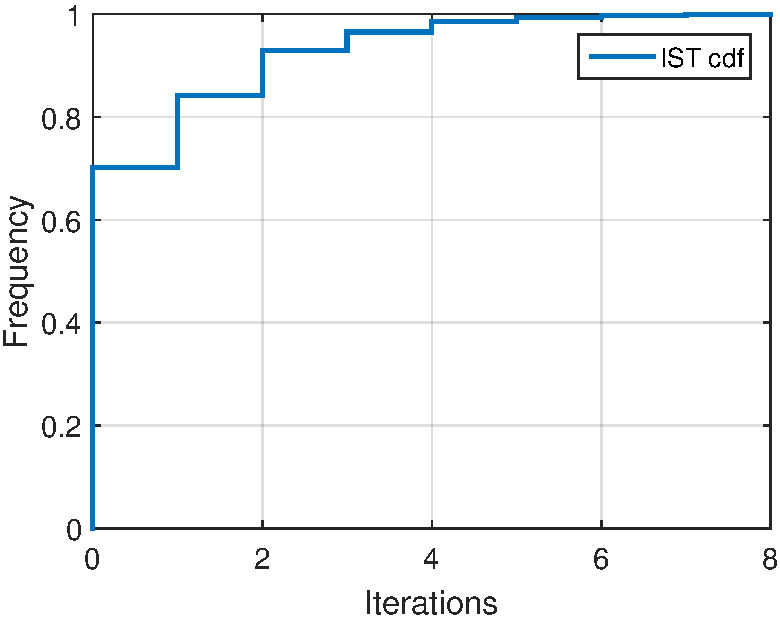
\includegraphics[scale=0.4]{figures/cdfnumber.pdf}
\label{fig:cdf}}\hspace{0.1cm}
\subfigure[Percent of error prediction by Fast-IST as
a function of threshold in window] {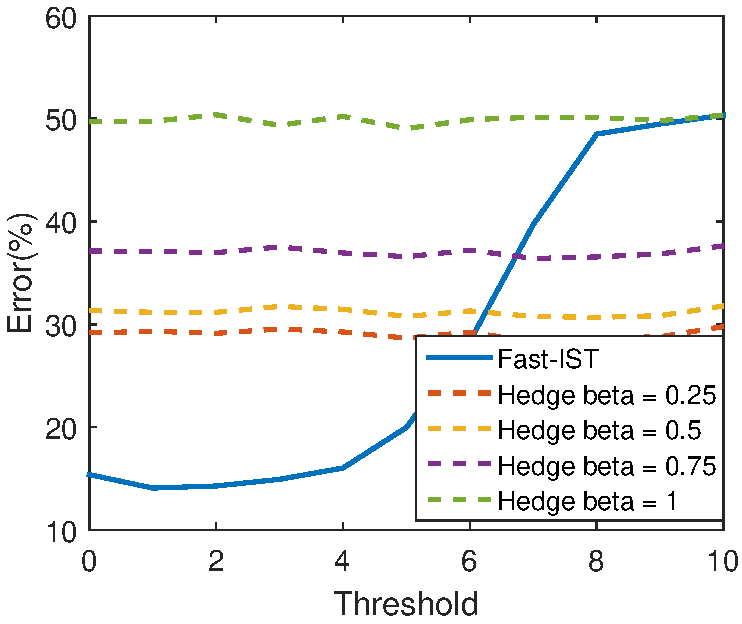
\includegraphics[scale=0.4]{figures/thresholdfactor.pdf}
\label{fig:threshold}}\hspace{0.1cm}
\subfigure[Percentage of error prediction by Fast-IST as a function of the number of training data] {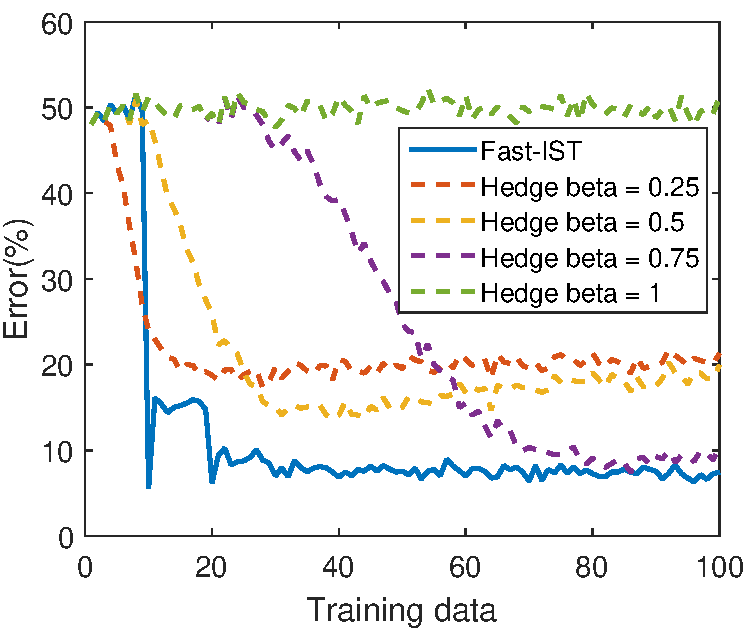
\includegraphics[scale=0.4]{figures/responsespeed.pdf}
\label{fig:speed}}
\caption{Evaluation of parameters and response speed}
\end{figure*}

\begin{figure*}[t]
\centering
\subfigure[Percent of error prediction by Fast-IST as a function of the correct prediction probability of the basic classifiers]{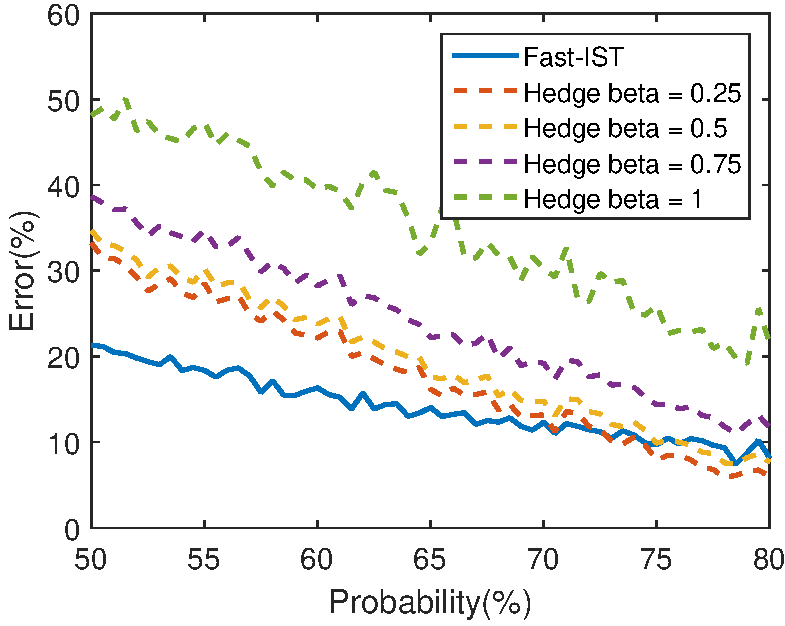
\includegraphics[scale=0.4]{figures/generalaccuracy.pdf}
\label{fig:saccuracy}}\hspace{0.1cm}
\subfigure[Running time of Fast-IST as a function of the number of training data]{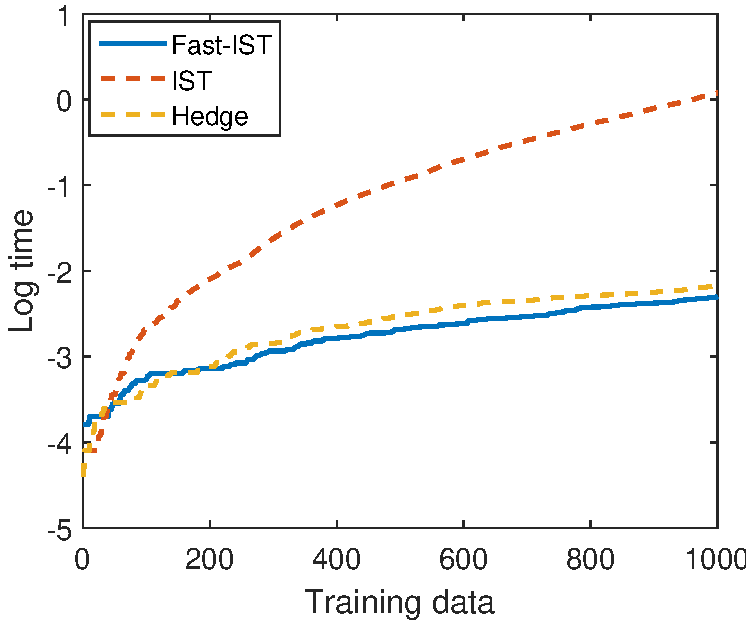
\includegraphics[scale=0.4]{figures/runningefficiency.pdf}
\label{fig:efficiency}}\hspace{0.1cm}
\subfigure[Percent of error prediction by Fast-IST in different class partitions]
{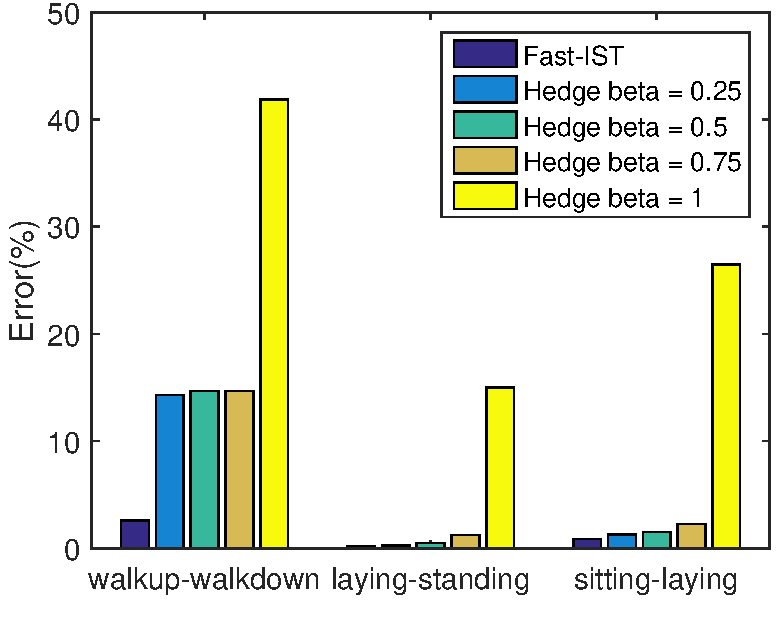
\includegraphics[scale=0.4]{figures/actualexp.pdf}
\label{fig:aaccuracy}}
%\subfigure[Number of no matching instances as a function of the number of trained data] {\includegraphics[scale=0.5]{figures/nomatchtime.pdf}
%\label{fig:eff2}}\hspace{0.1cm}
\caption{Evaluation of accuracy and efficiency}
\end{figure*}


%In the end of the last section, we propose two problems for online model adapting. In this section, we will address these two problems and put forward our algorithms: IST and Fast-IST.
\section{FAST-IST Framework}
FAST-IST is composed by 1) a data processing scheme to to schedule update; 2) model update by IST with a fixed number of iterations to bound computation cost, i.e., runs only a fixed number of pilot operations in each update.

\subsection{Data Processing to Control Update}
Given data stream $(\mathbf{x}_1, y_1), (\mathbf{x}_2, y_2), \ldots, (\mathbf{x}_n, y_n)$, we organize successive $l$ data points $\{(\mathbf{x}_i, y_i), i \in [l]\}$ into a batch $\mathbf{S}$  of length $l$.
We want to use these $l$ samples to measure the derivation between the current model and the expected model of the training data.
The idea comes from majority voting\cite{Ao:2016} \cite{penrose1946elementary}\cite{lam1997application}.
If most of data points in $\mathbf{S}$ can be fitted well by the current model, with high probability the minority unfitted samples in $\mathbf{S}$ come from noise. So the model is not necessary to update. But when the majority of data points violate the current model, the current model should be updated.

To measure how well the current model fits the data point $(\mathbf{x}, y)$, we can compare the error corresponding to the data point with the average error of the model. More specifically, suppose the current optimal model is $\mathbf{a}^t = (a_1, a_2, \ldots, a_m)$ and the average error is $\epsilon = \frac{1}{n}\sum_{i=1}^n\epsilon_i$. If
\begin{equation}
 -y\sum_{j=1}^m a_jG_j(\mathbf{x}) \geq \epsilon
\end{equation}
it indicates that the sample data can not be well fitted by the current model. Otherwise, the model is measured to fit the data well. Using this measure of fitness, the data filtering algorithm is as follows:
\begin{enumerate}
\item Divide stream into mini-batch $\{(\mathbf{x}_i, y_i), i \in [l]\}$ of size $l$
\item For all samples in $\{(\mathbf{x}_i, y_i), i \in [l]\}$, if $-y_i$ $\sum_{j=1}^m$ $a_jG_j(\mathbf{x}_i)$$\geq \epsilon $, count $(\mathbf{x}_i, y_i)$ as unfitted data point
\item If number of unfitted data point is less than threshold $T$, remove $\{(\mathbf{x}_i, y_i), i \in [l]\}$ from the stream.
\item Otherwise, update the  model by unfitted batch data.
\end{enumerate}

%Therefore, the selection of $l$ should take into account both noise and data transition. When $l$ is too small, some noise can not be detected which undermines the accuracy of the model. When $l$ is too large, the model can not quickly react to the change of data distribution.
%\subsection{Batch Data Smoothing}
%If the model needs to be updated, the batched data is smoothed to form two training instances. % For data with positive label, i.e., if $y_i =1$,
%\begin{equation}
%\left\{ \begin{array}{l}
%{\mathbf{x}_ + } = mean({\mathbf{x}_i},\forall {y_i} = 1)\\
%{\mathbf{x}_ - } = mean({\mathbf{x}_i},\forall {y_i} =  - 1)
%\end{array} \right.
%\end{equation}
%Then the model is updated by $\{(\mathbf{x}_+, 1)\}$, $\{(\mathbf{x}_-, -1)\}$ using fixed-iteration IST.

\subsection{Fixed-Iteration IST}
%In this section, the algorithms for efficient online updating $G$ using simplex and dual simplex are introduced. There are several polynomial time algorithms for solving linear programming such as ellipsoid algorithm \cite{KHACHIYAN198053} and inner point method \cite{Karmarkar:1984:NPA:800057.808695}, but they are not efficient online(??delete online?). An efficient way for online optimization is to utilize the optimal simplex tableau obtained in the previous step and conduct incremental simplex operations.
%Since the simplex tableau preserves the learned knowledge up to now, it can be leveraged to speed up the online computing, and the new optimal is generally not far from the previous optimal.

% Note that here rather than finding real optimal solution, we repeat pivot operation in constant many times to get an approximate solution where we make use the fact that the previous optimal solution is not far from new optimal solution.

%\subsection{Incremental Simplex tableau (IST)}

%\subsection{FAST-IST}
%IST can obtain the optimal solution for the optimization problem, but it has no guarantee of computational complexity since the number of pivot operation in simplex and dual simplex algorithm is not bounded. Also
Since the training data may be noisy, it is not necessary to always pursue the optimal model to fit the data. Thus, fixed-iteration IST is used in model update,  in which the number of iterations in Simplex is set to a constant $C$. %The solution is obtained after at most $C$ pivot operations. %More specifically, after doing at most $C$ rounds of pivot operation as IST, if solution is still non-optimal

\indent \indent \textbf{Deleting data:} When deleting past data, since simplex algorithm searches solution in the feasible region of the problem, the non-optimal solution is still feasible which can be used directly to form the combined classifier $G$.

\indent \indent \textbf{Adding data:} When adding new data, the dual simplex algorithm is applied to find the optimal solution. As dual simplex algorithm searches solution in the feasible region of the dual problem, the non-optimal solution may not satisfy all constraints of the problem. If there exists $a_j < 0$ in the non-optimal solution, we force $a_j = 0$ and normalize $\mathbf{a}$ to make the weights satisfy the constraints. %The combined classifier $G$ is constructed by the fixed weights.

%\subsection{Property Analysis}
%\paragraph{Feasibility} The feasibility for limiting the number of iterations in simplex and dual simplex algorithm in Fast-IST to approximate the optimal solution comes from
%\begin{itemize}
%\item Every time we change the system, the algorithm search for the optimal solution from the approximate solution in last system. Since only one sample of data is added every round, the new optimal solution should be close to the optimal solution in last round. If the former solution is a good approximation to the optimal one, it can not take too many iterations to get to the current optimal solution.
%\item In many cases, especially when basic classifiers $G_j$ have high accuracy, adding new data or removing old data do not cause the much weights updating. In this kind of rounds, $C$ is more than necessary number of iterations to update from last optimal solution to current optimal solution. Then this is a way of compensation for inaccurate solution in previous round to get rid of accumulating errors and this also utilize the fact that simplex algorithm has low average case complexity. So when $G_j$ have higher probability of correct classification, the smaller $C$ can be.
%\end{itemize}

\begin{theorem}
The computation complexity of Fixed-Iteration IST is $O(n^2)$, where $n$ is the size of the online data set.
\end{theorem}
\begin{proof}
The process of adding new data and deleting past data is symmetric and they have the same computational complexity. When the system changes, a pivot operation will visit every entry inside the columns corresponding to $\mathbf{x}_N$. The size of the simplex tableau is $n \times (m + 2n)$ and there are $m + n$ columns corresponding to $\mathbf{x}_N$. So it takes $O(Cn(m+n))$ steps for one update in Fixed-Iteration IST. Since $C$ is a constant and $m < n$, the computational complexity for once update is $O(n^2)$.
\end{proof}
As the average complexity for simplex algorithm is $O(n^3)$, The fixed iteration IST gives a $\Omega(n)$ speed up in each iteration. If we further consider the saving from data processing we will get an improvement of order $\Omega(l)$ for a carefully selected batch size $l$. There is a potential problem when $n$ is large since every time we use fixed iteration IST to approximate optimal solution, the error is accumulated when $n$ is large. This can undermine the efficiency of fixed iteration IST for later online training therefore we control the number of training data $n$ by alternately adding and deleting data to keep fast updating.

\section{Performance evaluation}
Performance evaluations of FAST-IST were conducted by both simulations and actual experimental data. Efficiency and accuracy are evaluated as the key performance for online adaptation.
\subsection{Settings of Simulation}
In simulations, basic classifiers ${G_j}$ are enumerated by random binary predictors with prediction accuracy ${p_j}$. Four aspects are mainly evaluated including 1) parameter impacts in Fast-IST; 2)responding speed;  3) accuracy;  and 4) running efficiency. The parameters of Fast-IST include the number of IST iterations, and the threshold for triggering update. Response speed is assessed by the number of online data needed for achieving stable ${a_j}$. %optimal adjustment. The less online data ${a_j}$ adjustment needs, the more sensitively online algorithms response to the incoming data.

The simulation uses $m$ basic classifiers and $n$ online training data. The correct probability of $m$ basic classifiers are set uniformly distributed from $55\%$ to $80\%$ to simulate BCs of different accuracy.  %in the offline training phase and ${a_j}$ were offline trained by linear programming.
In online phase, the correct probability  of each BC $p_j$ varies to simulate the impacts of the personalized features to the classifier model.

Fast-IST is compared with \emph{hedge algorithm}\cite{chaudhuri2009parameter}, which is widely used in online learning especially in online multi-kernel learning model.  In hedge algorithm, if some classifier makes a wrong prediction, when next sample of data comes, the weight of this classifier will be penalized by a ratio $0<\beta<1$. And the hedge algorithm predicts by weighting and summarizing all the basic classifiers' results.


%(2) 5 classifiers with the same correct probability and 100 training data are used to calculate average error percentage. The general accuracy is continuingly evaluated by varying the correct prediction probabilities of all classifiers from 50\% to 80\%.	 (3) In order to analyze running efficiency, running time of 1000 online data is recorded for 5 classifiers with different correct probability uniformly between 50\% and 80\%, the same correct probability distribution as that in (1).

%\indent \indent \textbf{Inner factor:} The number distribution of iterations in IST and window threshold will be analyzed in the subsection. 5 classifiers and 100 training data were used and we initially set all classifiers to predict with correct probability from 50\% to 80\% in the offline training phase and ${a_j}$ were offline trained by linear programming. In online phase, the prediction accuracy of $G_j$ varies for the incoming data to simulate the impacts of the personalized features to the classifier model.
%
%\indent \indent \textbf{Running efficiency:} Running time of 1000 online data for 5 classifiers, whose correct probability varying from 50\% to 80\%, of different online algorithms are compared. %Number of no matching instances are evaluated for evaluated 100 windows, with 10 instances for each window.
%
%\indent \indent \textbf{Response speed:} 50 classifiers with correct probability between 50\% and 80\% are used to analyze response speed of online algorithms on 100 training data. Good response speed means little online data is needed for ${a_j}$ optimal adjustment.
%
%\indent \indent \textbf{General accuracy:} For accuracy evaluation, we use 5 classifiers and 100 training data and varied the correct prediction
%probabilities of all classifiers from 50\% to 80\%.



%For algorithm comparison, the efficiency was compared to \emph{Linprog}, the standard linear programming solver in MATLAB, which is known to be one of the most efficient algorithm for linear programming using inner product method.

%For every experiments, training data $(\mathbf{x}_i, y_i)$ are added one by one and algorithm repeatedly computes the current combined classifier $G$ by trained data. We generate the prediction of $G_j$ by setting a probability $p_j$ and $G_j$ just randomly predicts with probability $p_j$ of correct prediction. Moreover in our experiments we set the maximum number of iterations in our algorithm to be 2 so we just do 2 pivot operation for every arriving data.



\subsection{Parameter Impacts to Fast-IST}

\subsubsection{Impacts of number of iterations}
At first, we verified how the number of iterations in Fast-IST will affect the performance. We investigated the number of iterations for achieving the optimal in IST.
The result, i.e., the distribution of iteration number in IST for achieving the optimal update is plotted in Fig.\ref{fig:cdf}, which is the cumulative distribution function (CDF) of the iteration number.
%when the base classifiers predicts randomly.
It can be seen that IST generally needs only a few iterations to update the model to the new optimal state. This indicates the validity of bounding the iteration times in Fast-IST, which will not much affect the performance.


\subsubsection{The threshold to trigger model update}. In Fast-IST, only when the numbers of wrong predictions in a batch exceeds a threshold $T$, will a new model update be triggered. How dose  $T$ affect the prediction accuracy of the combined classier after applied 100 instances of training data is shown Fig.\ref{fig:threshold}. In simulations the batch size is set to 10. It can be seen that, the optimal threshold is 2 or 3 when the batch size is 10. Setting higher threshold, although can reduce the triggering of update, but leads to much worse model accuracy.

\subsection{Responding Speed}
Responding speed is a key performance of online adaptation algorithms.
Fig.\ref{fig:speed} compares the response speed between Fast-IST and hedge of different parameters. It can be seen that Fast-IST adjusts $a_j$ more speedy than hedge. Hedge algorithms with small $\beta$, e.g. $0.25$ and $0.5$, also adapt quickly, because smaller $\beta$ adjusts weights more severely than bigger $\beta$. But hedge with smaller $\beta$ generally provides worse accuracy than Fast-IST. Fast-IST converges quickly, and there are  two obvious turnings points. The reason is that the batch length is 10. The turning points are where Fast-IST starts to correct the model weights.

\subsection{Accuracy}

Fig.\ref{fig:saccuracy} compares Fast-IST and hedge algorithm on the prediction accuracy. %In hedge algorithm, if some classifier makes a wrong prediction, when next sample of data comes, the weight of this classifier will be penalized by a ratio $0\le \beta \le 1$. Therefore, the model updating is very efficient with only one operation in each step, however, its optimality is not guaranteed.
In evaluation, the correct prediction probabilities of all basic classifiers are varying from 50\% to 80\%.
%The number of errors made by Fast-IST and hedge algorithm with different parameters, i.e., $\beta =$ 0.25, 0.5, 0.75 and 1 were compared.
It can be seen that Fast-IST have much less number of error prediction than hedge algorithm for all the $\beta$.

\subsection{Computation Efficiency}
%The running time of IST and Fast-IST are compared with that of Linprog. In each update, Linprog merged the newly collected training data and the old data to reevaluate the optimal weights. Instead, IST and Fast-IST used incremental updating. The running times of Linprog, IST and Fast-IST as a function of the size of online collected training data are plotted in Fig.\ref{fig:eff1}. It can seen that: as the number of online collected training data increases,  both Linprog and IST increase the running time but IST and Fast-IST are in general faster than Linprog. Linprog changes the internal algorithm after 500 samples. But note that the incoming online training data volume is generally small in each step, i.e., $<500$, in which case, IST and Fast-IST performance much more efficiently than Linprog.
The running time of Fast-IST are compared with hedge algorithm for 1000 online data. For clear comparison, we plot log results of running time in Fig.\ref{fig:efficiency}. It claims Fast-IST works a little faster than hedge algorithm and IST works highly more slowly than the other two algorithms.
%The reasons why IST and Fast-IST works greatly quickly are shown in Fig.\ref{fig:eff3}.
The reason why Fast-IST is even faster than hedge is that after $t$, i.e., the number of training data,  is larger than 100, update is rarely triggered in Fast-IST, since the model has fit the training data well. But hedge still updates frequently.
% It means $a_j$ is adjusted rarely, e.g. one update time in one window, when Fast-IST has been updated by more than 100 online data. Few update times brings about good running efficiency for Fast-IST.
%It can be found the number of no matching instances drops greatly, finally keeping smaller than 1, which equivalently represents highly few update times are needed for IST and Fast-IST.

%In Fig.\ref{fig:acc4}, the correct prediction probability of each basic classifier in online phase is modified slightly from its offline setting by adding a Gaussian noise to the expected correct prediction probability. So the online algorithms updates the combining weights to adapt to this modification. The prediction errors given by the updated models by IST, Fast-IST and hedge algorithm were compared. It can be seen that the updated model by IST and Fast-IST have much smaller prediction error than hedge algorithm for all $\beta =$ 0.25, 0.5, 0.75 and 1.

%So that IST provides online optimal updates and both IST and fast-IST provides much better prediction accuracy than the hedge-based algorithms.
\subsection{Evaluation by Activity Recognition Dataset}
\subsubsection{Experiment Settings}
%Abalone Data \cite{wu2009development} from open data set UCI \cite{Lichman:2013} is used to evaluate Fast-IST in actual experiment. The dataset is partitioned into two parts equally. One part is used to train basic classifiers offline and the other part works as personalized online data to update ${a_j}$. Each instance in Abalone Data is composed of 8 attributes and 3 classes $<$M, F, I$>$. We need to separately calculate error percent of $<$M, F$>$, $<$M, I$>$ and $<$F, I$>$. Five basic classifier are chosen, consisting of KNN \cite{peterson2009k}, Random forest (RF) \cite{liaw2002classification}, Naive Bayes (NB) \cite{rish2001empirical}, discriminant analysis classifier (DAC) \cite{scholkopft1999fisher} and SVM \cite{suykens1999least}.
%
%The prediction accuracy of Fast-IST and hedge algorithm for $<$M, F$>$, $<$M, I$>$ and $<$F, I$>$ are calculated and plotted in Fig.\ref{fig:aaccuracy}. The average prediction accuracy of five basic classifiers for three class partitions are shown in Table.\ref{tab}. It can be seen that Fast-IST and hedge algorithm indeed give more accurate predictions than all basic classifiers. And Fast-IST provides much better prediction accuracy than the hedge algorithms in all the three class partitions.

 Human Activity Recognition Using Smartphones Data Set from open data set UCI \cite{Lichman:2013} is used to evaluate Fast-IST in actual experiment.
 The database is composed of 7352 samples from 30 users with 561 types of sensor data from smartphones and 6 classes, $<$walking, walking-up, walking-down, sitting, standing, laying$>$. We separately calculated error percent $<$walking-up, walking-down$>$, $<$laying, standing$>$ and $<$sitting, standing$>$, which are hard to be classified. 187 basic KNN classifiers are chosen, each of which is trained on 3 types of sensor data.
  


The prediction accuracy of Fast-IST and hedge algorithm for $<$walking-up, walking-down$>$, $<$laying, standing$>$ and $<$sitting, standing$>$ are calculated and plotted in Fig.\ref{fig:aaccuracy}. The prediction accuracy distribution of 187 basic classifiers for three class partitions, i.e. mean, max, min, are shown in Table.\ref{tab}. It can be seen that Fast-IST and hedge algorithm indeed give much more accurate predictions than the basic classifiers. Especially, Fast-IST provides much better prediction accuracy than hedge algorithms in all the three classification problems. In classifying some hard cases such as walking up and walking down, Fast-IST provides significant accuracy improvement.

\begin{table}[!hbp]
\centering
\refstepcounter{table}\label{tab}
\begin{tabular}{|c|c|c|c|}
\hline
 & mean & max & min  \\
\hline
walkup-walkdown & 68.3253 & 86.0806 & 47.6190 \\
\hline
laying-standing & 63.0685 & 100 & 48.8358  \\
\hline
sitting-laying & 59.2011 & 99.0560 & 48.3952  \\
\hline
\end{tabular}
\caption{Accuracy of basic classifiers (\%)}
\end{table}

\section{Conclusion}
This paper has investigated online learning problem for adaptively personalizing learning model, where  multiple classifier combination is considered in particular. A simplex based online optimizing algorithm is proposed for both efficient and performance-guaranteed online model updating. We give the general IST algorithm and improved Fast-IST algorithm by proper data filtering and iteration bounding. Analysis shows that IST can guarantee the online optimal and Fast-IST provides near-optimal update with higher efficiency. The applications,  specification, and further optimization of IST and Fast-IST for particular problems, and the development of IST for batch updates will be investigated in future studies.

\section{Acknowledgment}
This work was supported in part by the National Natural Science Foundation
of China Grant No. 11671400, 61672524; the Fundamental
Research Funds for the Central University, and the Research
Funds of Renmin University of China, 2015030273; National Science Foundation of US awards Computing and Communication Foundations No.1565264 and Computer and Network Systems No.1618026.


%% The file named.bst is a bibliography style file for BibTeX 0.99c
\bibliographystyle{aaai}
\bibliography{aaai}

\end{document}



